\documentclass[11pt,letterpaper]{article}
\usepackage[lmargin=1in,rmargin=1in,tmargin=1in,bmargin=1in]{geometry}
\usepackage{../style/homework}
\usepackage{../style/commands}
\setbool{quotetype}{false} % True: Side; False: Under
\setbool{hideans}{false} % Student: True; Instructor: False

% -------------------
% Content
% -------------------
\begin{document}

\homework{15: Due 05/01}{True optimization is the revolutionary contribution of modern research to decision processes.}{George Dantzig}

% Problem 1
\problem{10} Find the maximum and minimum values for the function $z= 4x_1 + 5x_2$ on the region shown below. Be sure to fully justify that your answers are correct. 
	\[
	\fbox{
	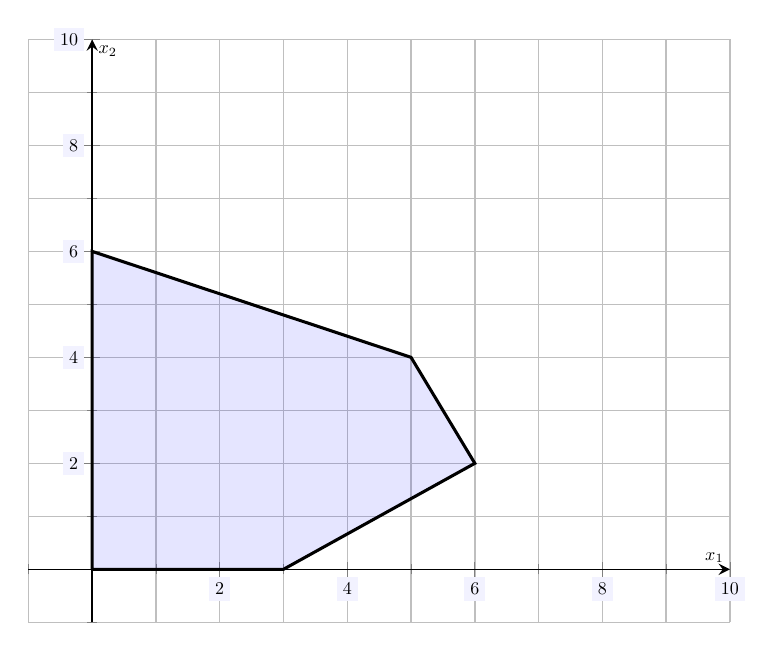
\begin{tikzpicture}[scale=1.3,every node/.style={scale=0.5}]
	\begin{axis}[
	grid=both,
	axis lines=middle,
	ticklabel style={fill=blue!5!white},
	xmin= -1, xmax=10,
	ymin= -1, ymax=10,
	xtick={0,2,4,6,8,10},
	ytick={0,2,4,6,8,10},
	minor tick = {-1,0,1,...,10},
	xlabel=\(x_1\),ylabel=\(x_2\),
	]
%	\addplot[domain= -1:10, line width=0.03cm] (x,5-x);
%	\draw[line width=0.03cm] (3,-10.5) -- (3,10.5);
	\draw[line width=0.01cm,fill= blue,opacity=0.1] (0,0) -- (0,6) -- (5,4) -- (6,2) -- (3,0) -- (0,0);
	\draw[line width=0.03cm] (0,0) -- (0,6) -- (5,4) -- (6,2) -- (3,0) -- (0,0);
	\end{axis}
	\end{tikzpicture}
	}
	\] \pspace

\sol First, observe that the region above is nonempty. For instance, the point $(0, 0)$ is in the region so that the region is not empty. The region is closed. Finally, because the region is contained in---for instance---the rectangle $[0, 6] \times [0, 6]$, the region is bounded. The function $z= 4x_1 + 5x_2$ is linear. Therefore, because the function $z$ is linear and the region is nonempty, closed, and bounded, the Fundamental Theorem of Linear Programming applies. But then we know that $z$ has a maximum and minimum on this region and that they must occur at a corner point. To find the maximum and minimum, we can simply find the value of $z$ at each corner point: \par
	\begin{table}[!ht]
	\centering
	\begin{tabular}{c|l}
	Corner Point & $z$ \\ \hline
	$(0, 0)$ & $z= 4(0) + 5(0)= 0 + 0= 0$ \\
	$(0, 6)$ & $z= 4(0) + 5(6)= 0 + 30= 30$ \\
	$(5, 4)$ & $z= 4(5) + 5(4)= 20 + 20= 40$ \\
	$(6, 2)$ & $z= 4(6) + 5(2)= 24 + 10= 34$ \\
	$(3, 0)$ & $z= 4(3) + 5(0)= 12 + 0= 12$
	\end{tabular}
	\end{table} \par
Therefore, the minimum value is $0$ and occurs at $(0, 0)$ and the maximum value is $40$ and occurs at $(5, 4)$. 
	\[
	\boxed{
	\begin{gathered}
	\min z= 0 \text{ at } (0, 0) \\
	\max z= 40 \text{ at } (5, 4)
	\end{gathered}
	}
	\]



\newpage



% Problem 2
\problem{10} Consider the function $z= 5x_1 - x_2$. Does this function has a maximum on the region shown below? If so, explain and find the maximum. If not, explain why. Answer the same question for the minimum of $z$ on the region shown below. 
	\[
	\fbox{
	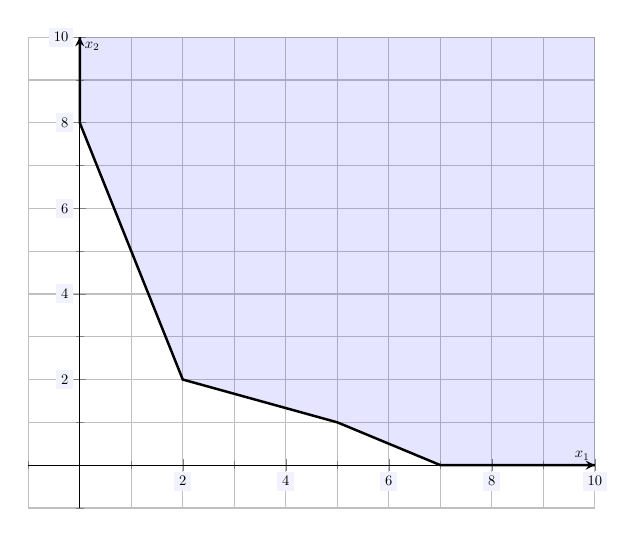
\begin{tikzpicture}[scale=1.05,every node/.style={scale=0.5}]
	\begin{axis}[
	grid=both,
	axis lines=middle,
	ticklabel style={fill=blue!5!white},
	xmin= -1, xmax=10,
	ymin= -1, ymax=10,
	xtick={0,2,4,6,8,10},
	ytick={0,2,4,6,8,10},
	minor tick = {-1,0,1,...,10},
	xlabel=\(x_1\),ylabel=\(x_2\),
	]
%	\addplot[domain= -1:10, line width=0.03cm] (x,5-x);
%	\draw[line width=0.03cm] (3,-10.5) -- (3,10.5);
	\draw[line width=0.01cm,fill= blue,opacity=0.1] (0,8) -- (0,10) -- (10,10) -- (10,0) -- (7,0) -- (5,1) -- (2,2) -- (0,8);
	\draw[line width=0.03cm] (0,10) -- (0,8) -- (2,2) -- (5,1) -- (7,0) -- (10,0);
	\end{axis}
	\end{tikzpicture}
	}
	\] \pspace

\sol First, observe that the region shown above is nonempty. For instance, the point $(2, 2)$ is in the region so that the region is not empty. The region is closed. The function $z= 5x_1 - x_2$ is linear. However, the region is \textit{not} bounded. For instance, the region contains the point $(x, x)$ for $x \geq 2$. But then the Fundamental Theorem of Linear Programming does not apply because the region is unbounded. Therefore, we will have to reason about the existence of maxima and minima for $z$ directly. \pspace

Observe that if $x_1$ is increased and $x_2$ is fixed, the function $z$ increases. If $x_1$ is fixed and $x_2$ is decreased, $z$ increases. Therefore, $z$ increases when we `move to the right and down.' But then if we choose the point $(x_1, 0)$ for $x_1 \geq 7$, this point is always in the region. But at such a point, we have $z(x_1, 0)= 5x_1 - 0= 5x_1$. But then choosing $x_1$ arbitrarily large, $z$ is arbitrarily large. Therefore, the function $z$ does not have a maximum on this region. \pspace

Observe that if $x_1$ is decreased and $x_2$ is fixed, the function $z$ decreases. If $x_1$ is fixed and $x_2$ is increased, the function $z$ decreases. Therefore, $z$ decreases when we `move to the left and up.' But there is no limit to how far `to the left and up' we can move in our region. For instance, the point $(x_1, x_2)= (0, x_2)$ is always in the region if $x_2 \geq 8$. But $z(0, x_2)= 5(0) - x_2= -x_2$. Because there is no limit to how large we can make $x_2$, there is no limit on how negative $z$ can be. Therefore, there is no minimum for the region. \pspace
	\[
	\boxed{
	\begin{gathered}
	\min z \colon \text{DNE} \\
	\max z \colon \text{ DNE}
	\end{gathered}
	}
	\]	


\end{document}